\section{Comparison with Existing Datasets}
\label{sec:comparison}

Table~\ref{tab:related_comparison} provides a comprehensive feature comparison
between \lucid{} and the most relevant existing language-annotated driving datasets.
Figure~\ref{fig:dataset_comparison} visualises the scale comparison by number of
language annotations.

\begin{table}[htbp]
  \centering
  \caption{Comparison of \lucid{} with existing language-annotated autonomous driving datasets.
  \cmark{} = supported, \xmark{} = not supported, $\sim$ = partially supported.}
  \label{tab:related_comparison}
  \renewcommand{\arraystretch}{1.25}
  \resizebox{\linewidth}{!}{%
  \begin{tabular}{@{}lccccccccc@{}}
    \toprule
    \textbf{Dataset} & \textbf{Scenarios} & \textbf{Lang.\ Ann.} & \textbf{Cities} & \textbf{Causal QA} & \textbf{Counterfactual} & \textbf{Multi-agent} & \textbf{Adv.\ Cond.} & \textbf{Planning Instruct.} & \textbf{Sensor} \\
    \midrule
    \rowcolor{cellblue}
    \textbf{\lucid{} (Ours)} & \textbf{12,847} & \textbf{847,293} & \textbf{6} & \cmark & \cmark & \cmark & \cmark & \cmark & C+L+R \\
    DriveLM~\cite{sima2023drivelm}           & 4,807  & 150,000  & 1 & $\sim$ & \xmark & $\sim$ & \xmark & $\sim$ & C+L \\
    NuScenes-QA~\cite{qian2024nuscenes_qa}   & 34,149 & 459,941  & 6 & \xmark & \xmark & \xmark & \xmark & \xmark & C+L+R \\
    NuPrompt~\cite{wu2024nuprompt}           & 34,149 & 35,367   & 6 & \xmark & \xmark & \xmark & \xmark & \xmark & C+L+R \\
    DRAMA~\cite{malla2023drama}              & 14,000 & 17,785   & 1 & \xmark & \xmark & $\sim$ & \xmark & \xmark & C \\
    BDD-X~\cite{kim2018textual}              & 26,000 & 26,000   & $>$3 & \xmark & \xmark & \xmark & \xmark & \xmark & C \\
    HAD~\cite{chen2019had}                   & 5,675  & 45,000   & 1 & \xmark & \xmark & \xmark & \xmark & \cmark & C \\
    STRIDE-QA~\cite{wu2024stride}            & N/A    & 20,000   & 1 & \xmark & \xmark & \xmark & \xmark & \xmark & C+L \\
    Rank2Tell~\cite{rank2tell2024}           & 7,478  & 10,000   & 1 & \xmark & \xmark & $\sim$ & \xmark & \xmark & C+L \\
    CoVLA~\cite{covla2024}                   & 9,000  & 12,000   & 1 & \xmark & \xmark & \xmark & \xmark & \xmark & C \\
    WEDGE~\cite{wedge2024}                   & 5,000  & 5,000    & 3 & \xmark & \xmark & \xmark & \cmark & \xmark & C \\
    IEDD~\cite{iedd2024}                     & 8,000  & 8,000    & 2 & \xmark & \xmark & \xmark & $\sim$ & \xmark & C+L \\
    Box-QAymo~\cite{boxqaymo2024}            & N/A    & 90,000   & 1 & \xmark & \xmark & \xmark & \xmark & \xmark & C+L \\
    PotentialRiskQA~\cite{potentialrisk2024} & 6,000  & 6,000    & 1 & \xmark & \xmark & $\sim$ & \xmark & \xmark & C \\
    CARScenes~\cite{carscenes2024}           & 14,000 & 14,000   & 2 & \xmark & \xmark & \xmark & \xmark & \xmark & C \\
    \bottomrule
    \multicolumn{10}{l}{\footnotesize C = camera, L = LiDAR, R = radar. Partial support ($\sim$) indicates indirect or limited coverage.} \\
  \end{tabular}%
  }
\end{table}

\begin{figure}[htbp]
  \centering
  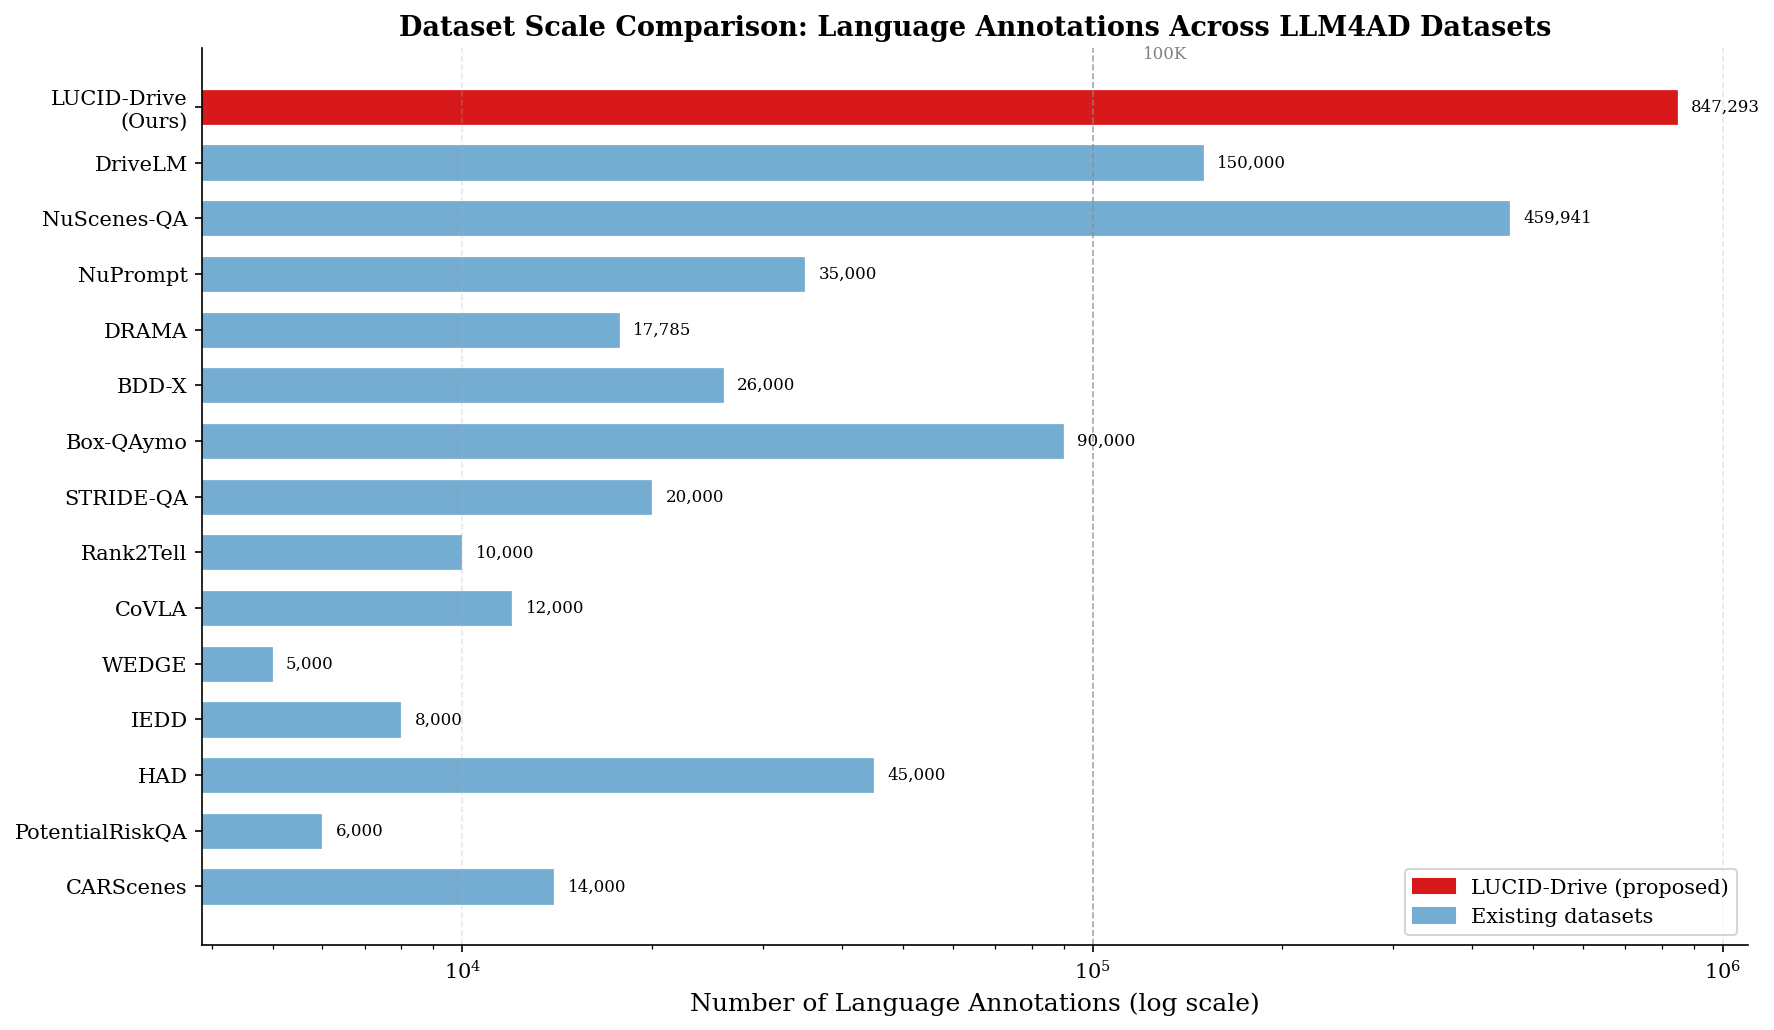
\includegraphics[width=\linewidth]{figures/dataset_comparison.png}
  \caption{Scale comparison by number of language annotations across LLM4AD datasets
  (log scale). \lucid{} provides the largest collection of language annotations (847,293),
  nearly twice that of NuScenes-QA (459,941), the previous largest.}
  \label{fig:dataset_comparison}
\end{figure}

\subsection{Key Differentiators}
\label{ssec:comparison_diff}

\textbf{Causal reasoning annotations.} \lucid{} is the only dataset providing
structured causal chain QA pairs (312,456) where answers explicitly model the
causal structure of driving events. DriveLM provides graph-structured VQA chains
that partially capture causality ($\sim$), but these are limited to three fixed
question types (perception, prediction, planning) and do not model counterfactual
hypotheses.

\textbf{Counterfactual reasoning.} No existing dataset provides dedicated counterfactual
QA pairs. \lucid{} introduces 198,327 counterfactual pairs with physical-plausibility
validation, enabling the first systematic evaluation of counterfactual reasoning in AD.

\textbf{Scale of planning instructions.} HAD provides highway-specific advice
but is limited to a single location and driving context. \lucid{} provides 156,832
planning instructions spanning all five scenario categories and six cities.

\textbf{Sensor richness.} NuScenes-QA and NuPrompt are built on the nuScenes
sensor suite (C+L+R), providing comparable sensor diversity to \lucid{}.
However, their annotations focus entirely on object-level perception rather than
causal or counterfactual reasoning.

\textbf{Geographic and condition diversity.} WEDGE and IEDD provide targeted
adverse-condition coverage but in limited geographic contexts (1--3 cities).
\lucid{} combines six-city geographic diversity with seven-weather and four-lighting
coverage, the most comprehensive condition matrix in the literature.

\textbf{Multi-agent grounding.} \lucid{}'s agent intention labels (412,847 instances)
and causal chain annotations explicitly represent multi-agent interactions in language,
enabling training and evaluation of models that reason about other agents' intentions
and their effects on ego-vehicle decisions.
